\section{The Fourier Transform\label{sec:fourier}}
\subsection{Definition}
The Fourier Transform (FT) decomposes a function
from the space or time domain into the frequency domain.
If we view a function $g$ as an infinite-dimensional vector,
then FT transforms $g$ from a representation in the standard basis
to one in a basis of complex sinusoids.
It can be defined as follows:
%
\begin{equation}
     \hat g(f) = \int_{-\infty}^{\infty} g(x) \cdot e^{-i 2 \pi f x} dx
\end{equation}
%
A continuous function $g: \mathbb{R} \rightarrow \mathbb{R}$
can be described as a sum of waves (in this case sinusoids).
FT can tell us the presence of each frequency in the function.

It can be hard to develop an intuition for the transform.
An excellent visual representation is provided by \cite{3blue} in video form,
which we can somewhat replicate with a sequence of images in figure \ref{fig:winding}.
$g$ is wound around zero in the complex plane with periodicity corresponding to $f$,
and $\hat g(f)$ can be viewed as the ``center of mass'' for this winding, given by an integral.
If a frequency is present in $g$,
winding with the same periodicity will cause the integral to deviate from zero.
\begin{figure}
    \centering
    \begin{subfigure}[b]{0.45\textwidth}
    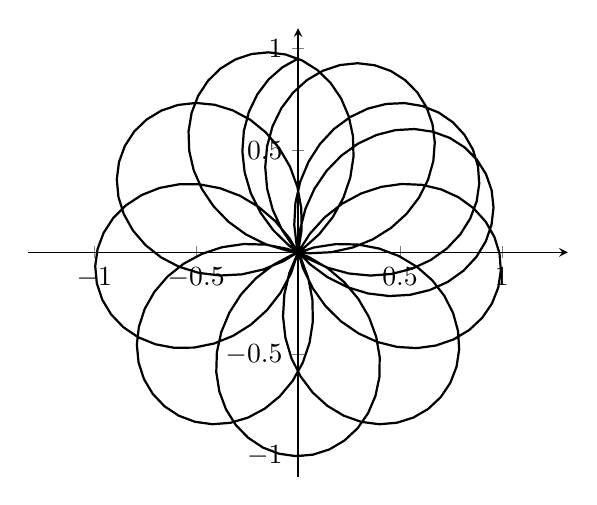
\begin{tikzpicture}
        \begin{axis}[axis lines = middle, trig format plots = rad, axis equal, xmin = -1.1, xmax = 1.1, ymin = -1.1, ymax = 1.1]
            \addplot [domain = 0:4*pi*2, samples = 300, thick]({(sin(1.30*x))*sin(x)},{(sin(1.30*x))*cos(x)});
        \end{axis}
    \end{tikzpicture}
    \caption{Winding frequency: $1.30$\label{fig:windinga}}
    \end{subfigure}
    \begin{subfigure}[b]{0.45\textwidth}
    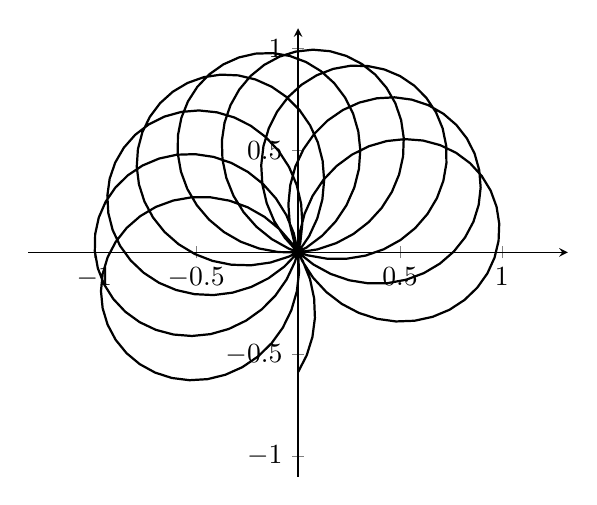
\begin{tikzpicture}
        \begin{axis}[axis lines = middle, trig format plots = rad, axis equal, xmin = -1.1, xmax = 1.1, ymin = -1.1, ymax = 1.1]
            \addplot [domain = 0:4*pi*2, samples = 300, thick]({(sin(1.15*x))*sin(x)},{(sin(1.15*x))*cos(x)});
        \end{axis}
    \end{tikzpicture}
    \caption{Winding frequency: $1.15$\label{fig:windingb}}
    \end{subfigure}
    \begin{subfigure}[b]{0.45\textwidth}
    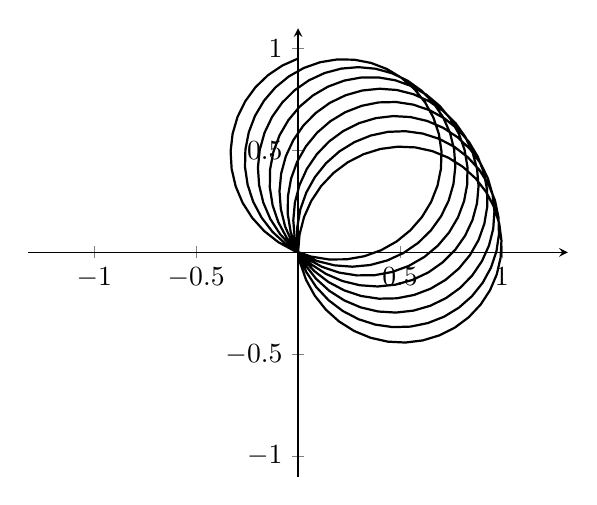
\begin{tikzpicture}
        \begin{axis}[axis lines = middle, trig format plots = rad, axis equal, xmin = -1.1, xmax = 1.1, ymin = -1.1, ymax = 1.1]
            \addplot [domain = 0:4*pi*2, samples = 300, thick]({(sin(1.05*x))*sin(x)},{(sin(1.05*x))*cos(x)});
        \end{axis}
    \end{tikzpicture}
    \caption{Winding frequency: $1.05$\label{fig:windingc}}
    \end{subfigure}
    \begin{subfigure}[b]{0.45\textwidth}
    \begin{tikzpicture}
        \begin{axis}[axis lines = middle, trig format plots = rad, axis equal, xmin = -1.1, xmax = 1.1, ymin = -1.1, ymax = 1.1]
            \addplot [domain = 0:4*pi*2, samples = 300, thick]({(sin(x))*sin(x)},{(sin(x))*cos(x)});
        \end{axis}
    \end{tikzpicture}
    \caption{Winding frequency: $1.00$\label{fig:windingd}}
    \end{subfigure}
    \caption{Plots of $sin(x)$ wound around zero in the complex plane with different winding ``speeds''.
    The integral of (\ref{fig:windingd}) will deviate to the right in a much greater degree than the others.
    \label{fig:winding}}
\end{figure}

The Fourier inversion theorem states that,
for certain functions,
the inverse of the Fourier transform can be obtained by:
\begin{equation}
     g(x) = \int_{-\infty}^{\infty} \hat g(f) \cdot e^{i 2 \pi f x} df
\end{equation}
This can be used to build a function from a description of its sinusoid components.

In real-world applications, we usually aren't working with continuous functions.
Typically we have a sequence of uniformly spaced samples approximating a recorded signal,
and we wish to compute something FT-like for this.
We cannot compute the FT of such a signal,
but we can approximate it using the Discrete Fourier Transform (DFT):
%
\begin{equation}
    X(k) = \sum_{n = 0}^{N - 1} x(n) \cdot e^{-i 2 \pi kn / N}
\end{equation}
%
The DFT is also an invertible, linear transformation.
The Inverse Discrete Fourier Transform (IDFT) is defined as:
\begin{equation}
    x(n) = \sum_{k = 0}^{N - 1} X(k) \cdot e^{i 2 \pi kn / N}
\end{equation}
%
We wish to write an efficient reversible algorithm
that computes the DFT when run in the forward direction
and computes the IDFT when run backwards.
